\section{TCGAbiolinks: An R package to download and analyze data from TCGA}


 Integrative analysis of genomic big-data collections from public databases such as The Cancer Genome Atlas (TCGA) can advance knowledge and lead to new discoveries in cancer research.  However, the data retrieval from TCGA is a cumbersome and time-consuming task. The TCGABiolinks Bioconductor package allows to query, download and perform integrative analysis with TCGA data, combining computer science and statistical methods thus authoring reproducible analysis. 
  Case studies are reported on various cancer system biology applications including a complete downstream analysis with LGG and GBM, by means of gene expression data,  methylation data and integration of both data.
  The analysis layer and visualization layer were combined into a reusable workflow. 
  The TCGABiolinks package is released under GPL3 License within Bioconductor project. The source code and vignette are freely available at \url{http://bioconductor.org/packages/TCGAbiolinks/}.
  
  The Cancer Genome Atlas (TCGA) has made the effort to collect a wide range of different data sets and at the same time offers an API to access these data sets. However, this can only be seen as the first step towards allowing different researchers access to these data sets. The question that needs to be answered next is how can we best access, prepare and then analyze the data most efficiently given a specific problem. 
The number of publications in pubmed related to TCGA (July 2015) is 1517 and the number of publications per year has increased every year since its conception (Figure~\ref{NAR-fig1}).

\begin{figure}
\centering
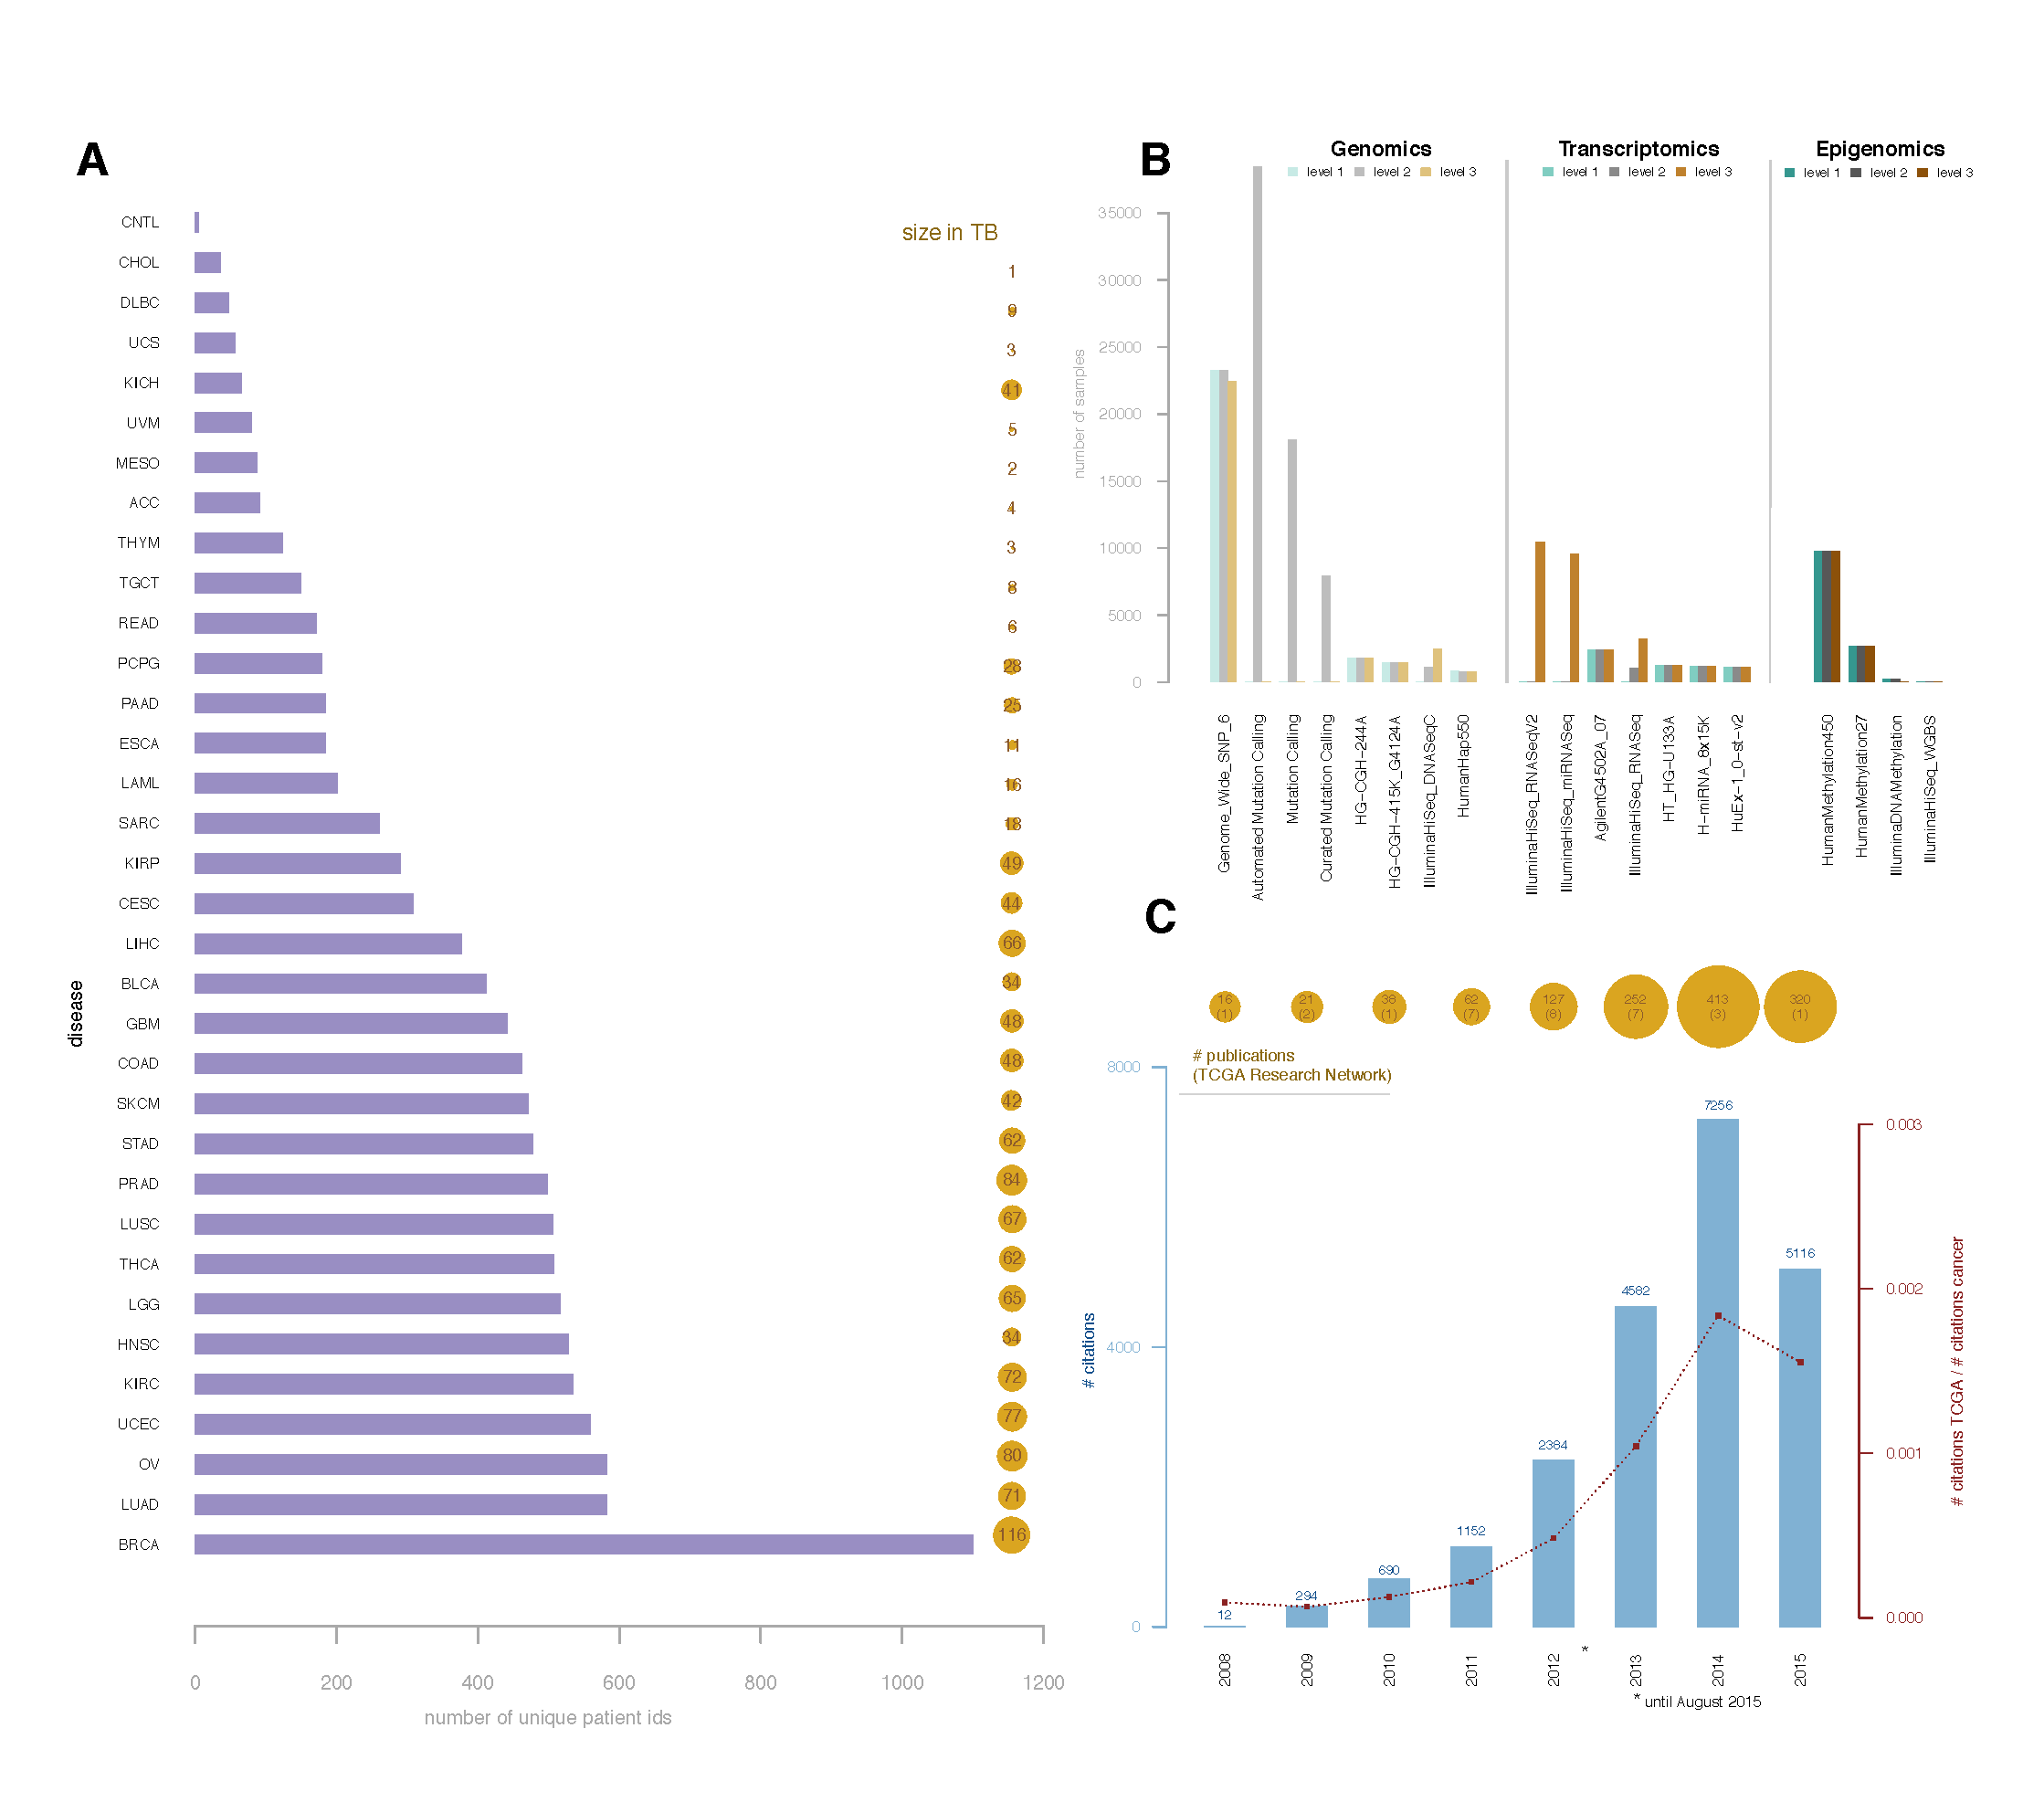
\includegraphics[width=1.0\textwidth]{images/figure1_draft2.pdf}
\caption[]{TCGA data overview. (A) bars represent number of patients by disease; bubbles represent the available data size in TB by disease; (B) number of samples by platform and by level, grouped by type: genomic, transcriptomic and epigenomic. (C) Barplot: number of citations for TCGA papers. Bubble plot: number of TCGA papers, in parenthesis the number of papers published by the TCGA Research Network. Source: Scopus search for 'TCGA', adding TCGA Research Network papers that were not found during this search.}
\label{fig:my_label}
\end{figure}

This increased publication frequency does not only imply that the number of researchers that use TCGA data increases but it also attracts researchers new to these data sets.
There are two distinct groups of researchers such as beginners-intermediate and advanced and they are very different in nature. 
While the former still spends a large amount of time on downloading and pre-processing the data for the subsequent analyses, the latter first has to understand both the different data types and the analyses typically applied to them. The usual approach for obtaining help for both types of users consists in asking questions on portals such as \textit{stackoverflow.com}, \textit{support.bioconductor.org} or \textit{biostars.org}.\\

%%%%%%%%% Reduce state of art in one paragraph %%%%%%%%% 

Recently, different tools to retrieve TCGA datasets have been made available, these include TCGA-Assembler  (\cite{Zhu14}), CGDS-R (\cite {gao2013integrative}), cBioPortal \cite{cerami2012cbio}, canEnvolve (\cite{samur2013canevolve}), BioXpress \cite{wan2015bioxpress},  Firehose \footnote{http://gdac.broadinstitute.org}, and
RTCGAtoolbox~\cite{samur2014rtcgatoolbox}.
% Reorganize the features in 3 categories
The features for each tool can be divided into four representative categories (i) downloader, ii) data integration and analysis, and iv) visualization. 
The fist category comprises tools that mainly download cancer genomics data: TCGA-Assembler, the Bioconductor package CGDS-R and cBioPortal. 
% TCGA-Assembler written in R apply a recursive algorithm to retrieve the URLs of all data files. This open software package automates and streamlines the acquisition, assembling, and processing of public TCGA data. It can be integrate with R libraries for downstream analysis.
% CGDS-R, at the moment, the only tool available on CRAN or Bioconductor provides a basic set of R functions for querying the Cancer Genomic Data Server (CGDS) hosted by the Computational Biology Center (cBio).
% cBioPortal is a web portal for interactively exploring multidimensional cancer genomics data sets in the context of clinical data and biologic pathways. It allows explorative data analysis, and provides simple download of small data slices.
% A key feature of the cBio portal is ease of use, if you want to explore a pathway of interest in one or more cancer types, but to download raw mRNA expression files or full segmented copy number files, it's not suitable.
The second category includes tools that focus on data analysis and integration, such as Firehose, canEnvolve or BioXpress.
% canEnvolve contains integrated data from 90 studies involving more than 10000 patients. Data analysis are involved at different levels: 1) mRNA/miRNA and copy number 2) integrative analysis between genes, protein and copy number 3) network and pathway analysis 4) survival analysis. It is a web portal and can be a limit for researchers that want to analyse data in an R environment. \\
% BioXpress \cite{wan2015bioxpress} database stores RNA-seq data from several publicly available sources, among them TCGA, and through standardize method identifies the expression levels of the genes. 
% The third category includes tools to download, analyse, and integration data, such as Firehose.
% The Firehose has been developed to download and analyze (e.g. GISTIC 2.0 and MutSig), in an automated and reproducible way, the data generated by TCGA. The results are  available via a website.  However, it has several limitations to access the data and it is not easily integrated with programming environments for downstream analysis(\cite{samur2014rtcgatoolbox}). \\
The third category comprises tools to download, analyze ,integration and visualization such as RTCGA-Toolbox.
% RTCGAToolbox (\cite{samur2014rtcgatoolbox}) was designed, using R programming language,  
to systematically access Firehose pre-processed data and to perform basic analysis and visualization.

TCGA provides unprecedented opportunities to interrogate the genome and epigenome of normal and tumor tissues proving public access to more than 20 tumor types. Markedly however, preparing these data for various  analysis pipelines 
is a time-consuming task as the biological information is stored in different formats through a large number of files.

Despite the existence of some integrative TCGA-specific software packages, few are available from Bioconductor and none or few of them perform integrative analysis. 
Being part of the Bioconductor project ensures the high-quality, well documented and interoperable software and the possibility of integration with hundreds of available packages.
%,  helping the user to work with different packages and analysis.


We introduce \textit{TCGAbiolinks} an R/Bioconductor package for integrative analysis with TCGA data.
The aim of TCGAbiolinks is four-fold: i) facilitate the data retrieval, ii) prepare the data using the appropriate pre-processing strategies, iii) provide the means to carry out different standard analyses and iv) allow the user to download a specific version of the data and thus to easily reproduce earlier research results.

In more detail, the package provides multiple methods for analysis (e.g., differential expression analysis, identifying differentially methylated regions) and methods for visualization (e.g., survival plots, starburst plots) in order to easily develop complete analysis pipelines. An example of the package overflow is presented in Figure \ref{NAR-fig3}. %flux


%%%%%%%%% NEW FIGURE

 \tikzstyle{texto} = [above, 
 					  text width=6em, 
                      text centered,
                      font=\normalsize]

\tikzstyle{start} = [rectangle,
                     minimum size=6mm,%rounded corners=3mm,
					 very thick,
                     draw = black!50, 
                     top color = white,
                     bottom color = black!20,
                     font=\itshape\footnotesize,
                     drop shadow, 
                     align=center]
                     
\tikzstyle{fail} = [rectangle, 
					rounded corners, 
                    minimum width=3cm, 
                    minimum height=1cm,
                    text centered,
                    font=\itshape\footnotesize, 
                    draw=black, 
                    fill=red, 
                    text=white,  
                    drop shadow]
                    
\tikzstyle{success} = [rectangle, 
					   rounded corners, 
                       minimum width=3cm, 
                       font=\itshape\footnotesize,
                       minimum height=1cm,
                       text centered, 
                       draw=black,
                       fill=green!70!black!70, 
                       text=white,  
                       drop shadow]
\tikzstyle{process} = [rectangle, 
					   minimum width=1cm, 
                       minimum height=0.5cm, 
                       text centered, 
                       text width=3cm, 
                       font=\itshape\footnotesize,
                       draw=black, 
                       fill=black!40, 
                       text=white,drop shadow]
\tikzstyle{decision} = [diamond, 
						minimum width=0.5cm, 
                        minimum height=0.5cm,
                        font=\itshape\footnotesize,
						text centered, 
                        draw=black,
						top color = white,
                        bottom color = yellow!80, 
                        text=black, 
                        drop shadow]
                        
\tikzstyle{arrow} = [thick,->,>=stealth,-latex',draw,rounded corners]
\tikzstyle{cloud} = [draw, 
					 ellipse,
					 rounded corners = 3mm,
                     very thick,
                     draw           = orange!50, 
                     top color      = white,
                     bottom color   = orange!20,
                     font           = \itshape\footnotesize,
                     node distance  = 4cm,
                     minimum height = 1em,
                     drop shadow]


\begin{figure}[!h]
 \begin{center}
 \begin{tikzpicture}[node distance = 1.5cm, 
 					 auto, shorten >=1pt,
                     thick,font=\itshape\footnotesize,
                     ->,
                     >=stealth']
 \linespread{0.8}{

 \node (clinic) [start]{TCGAquery\_clinic};
 \node (start) [start, below of=clinic,yshift=0.5cm] {TCGAquery};
 \node (download) [start, below of=start,yshift=0.5cm] {TCGAdownload};
 \node (prepare) [start, below of=download,yshift=0.5cm] {TCGAprepare};
 \node (version) [start, below of=prepare,yshift=0.5cm] { TCGAquery\_version};

 \node (coxnet) [start, right of=clinic, yshift=0cm,xshift = +1.5cm] {survivalCoxNET};
 \node (survival) [start, right of=start, yshift=0cm,xshift = +1.5cm] {survival};
 \node (eacomplete) [start, right of=download, yshift = 0cm,xshift = +1.5cm] {EAcomplete};
 \node (eabarplot) [start, right of=eacomplete, xshift = +1cm] {EAbarplot};
 \node (dea) [start, right of=prepare,yshift = 0cm, xshift = +1.5cm] {DEA};
 \node (dmr) [start, right of=version, xshift = +1.5cm,yshift = 0cm] {DMR};

 \node (starburst) [start, right of=dmr, xshift = 1cm,yshift = 0.3cm] {starburst};

 \tikzstyle{texto} = [above, text width=6em, text centered,font=\normalsize]

 \path [arrow] (start) -- (download);
 \path [arrow] (download) -- (prepare);
 \path [arrow] (prepare) -- (eacomplete);
 \path [arrow] (eacomplete) -- (eabarplot);
 \path [arrow] (prepare) -- (dea);
 \path [arrow] (prepare) -- (dmr);
 \path [arrow] (dmr) -- (starburst);
 \path [arrow] (dea) -- (starburst);
 \draw (prepare) edge[out=0,in=180,->,color=red!80!black] (dmr);
 \draw (prepare) edge[out=0,in=180,->,color=green!60!black] (dea);
 \draw (prepare) edge[out=0,in=200,->,color=green!60!black] (eacomplete);
 \draw (prepare) edge[out=0,in=180,->,color=green!60!black] (coxnet);
 \draw (clinic) edge[out=0,in=180,->,color=blue!80!black] (coxnet);
 \draw (clinic) edge[out=0,in=180,->,color=blue!80!black] (survival);
 \path [arrow,color=blue!80!black] (clinic) -- (survival);

 }
 % Background
 \begin{pgfonlayer}{background}
   \begin{pgfonlayer}{background}
         % Compute a few helper coordinates
         \path (start.west |- start.north)+(-0.5,0.5) node (a) {};
		 \path (prepare.south -| prepare.east)+(+0.3,-0.2) node (b) {};
		 \path (clinic.west |- clinic.north)+(-0.5,0.6) node (a) {};
         \path (dmr.south -| prepare.east)+(+0.3,-0.2) node (b) {};
         \path (starburst.south -| eabarplot.east)+(+0.25,-0.55) node (c) {};
         \path (eabarplot.west |- survival.north)+(-0.2,1.65) node (d) {};
		 \path (dmr.south -| coxnet.east)+(+0.2,-0.225) node (e) {};
         \path (coxnet.west |- survival.north)+(-0.2,1.65) node (f) {};
         \path[fill=cyan!20,rounded corners, draw=black!50, dashed]
             (a) rectangle (b);
         \path (dmr.west |- clinic.north)+(-0.2,1.0) node (a) {};
         \path (dmr.south -| starburst.east)+(+0.2,-0.3) node (b) {};
         \path[fill = yellow!30,
               rounded corners, 
         	   draw = black!50, dashed]
             (e) rectangle (f);
         \path (clinic.west |- clinic.north)+(0.65,0.3) node (u1)[texto,font=\normalsize]
       {\normalsize{Data functions}};
         \path (survival.north |- dmr.east)+(+0.0,+4.65) node (u1)[texto,font=\normalsize] {\normalsize{Analysis}};
          \path[fill = magenta!20,
                rounded corners, 
                draw = black!50, 
                dashed]
            (d) rectangle (c);
         \path (starburst.north |- starburst.east)+(-0.1,+4.35) node (u1)[texto,font=\normalsize] {\normalsize{Visualize}};
 	\end{pgfonlayer}
 \end{pgfonlayer}

 \end{tikzpicture}
 \end{center}
 \caption[Example of TCGAbiolinks workflow]{Example of a complete workflow using TCGAbiolinks: functions were divided in three groups - data (blue), analysis (yellow) and visualize (green). Green arrows represent expression data, red arrows methylation data and blue arrows clinical data. The function TCGAquery searches for TCGA data using as input the tumor type, platform, level, version of the data and list of samples. The output of TCGAquery will be downloaded with TCGAdownload. TCGAprepare will read the data and prepare the data into a SummarizedExperiment object.%, if save parameter is true the final object is saved. 
 Afterwards, downstream analyses can be performed. For example for methylation data, TCGAanalyze\underline{\space}DMR can be used for Differential methylation analysis. Differential expression analysis can be carried out with TCGAanalyze\_DEA. Integrative visualization of  both results  is possible  using TCGAvisualize\underline{\space}starburst.} 
 \label{NAR-fig3} %flux
 \end{figure}




\section{MATERIALS AND METHODS}
\subsection{The TCGAbiolinks package}

\textit{TCGAbiolinks} is composed of seven functions / layers that can be grouped into three levels: DATA, APPLICATION and SOCIAL.
%This idea was inspired to Open Systems Interconnection model (OSI Model) ISO/OSI layers, and like ISO OSI the data passes severals levels from TCGA ftp folders, where TCGA's data are located, to application level. Furthermore we added a social level more.
These functions can be used independently but also in combination to provide the user with fully understandable analysis pipelines applied to TCGA data.

%\begin{itemize}
%\item DATA: \textit{TCGAquery}, \textit{TCGAdownload}, \textit{TCGAprepare}
%\item APPLICATION: TCGAanalyze, TCGAvisualize
%\item SOCIAL: TCGAinvestigate, TCGASocial
%\end{itemize}

%\begin{figure}[!h]
%\begin{center}
%\includegraphics[width=.9\linewidth]{images/TCGAbiolinks_levels.png}
%\includegraphics[width=.9\linewidth]{images/TCGAbiolinks_levels2.png}
%\end{center}
%\caption{TCGAbiolinks layered functions levels}
%\label{NAR-fig2}
%\end{figure}


\subsection{Outline of the TCGAbiolinks package functionalities.}
\begin{figure*}
\centering
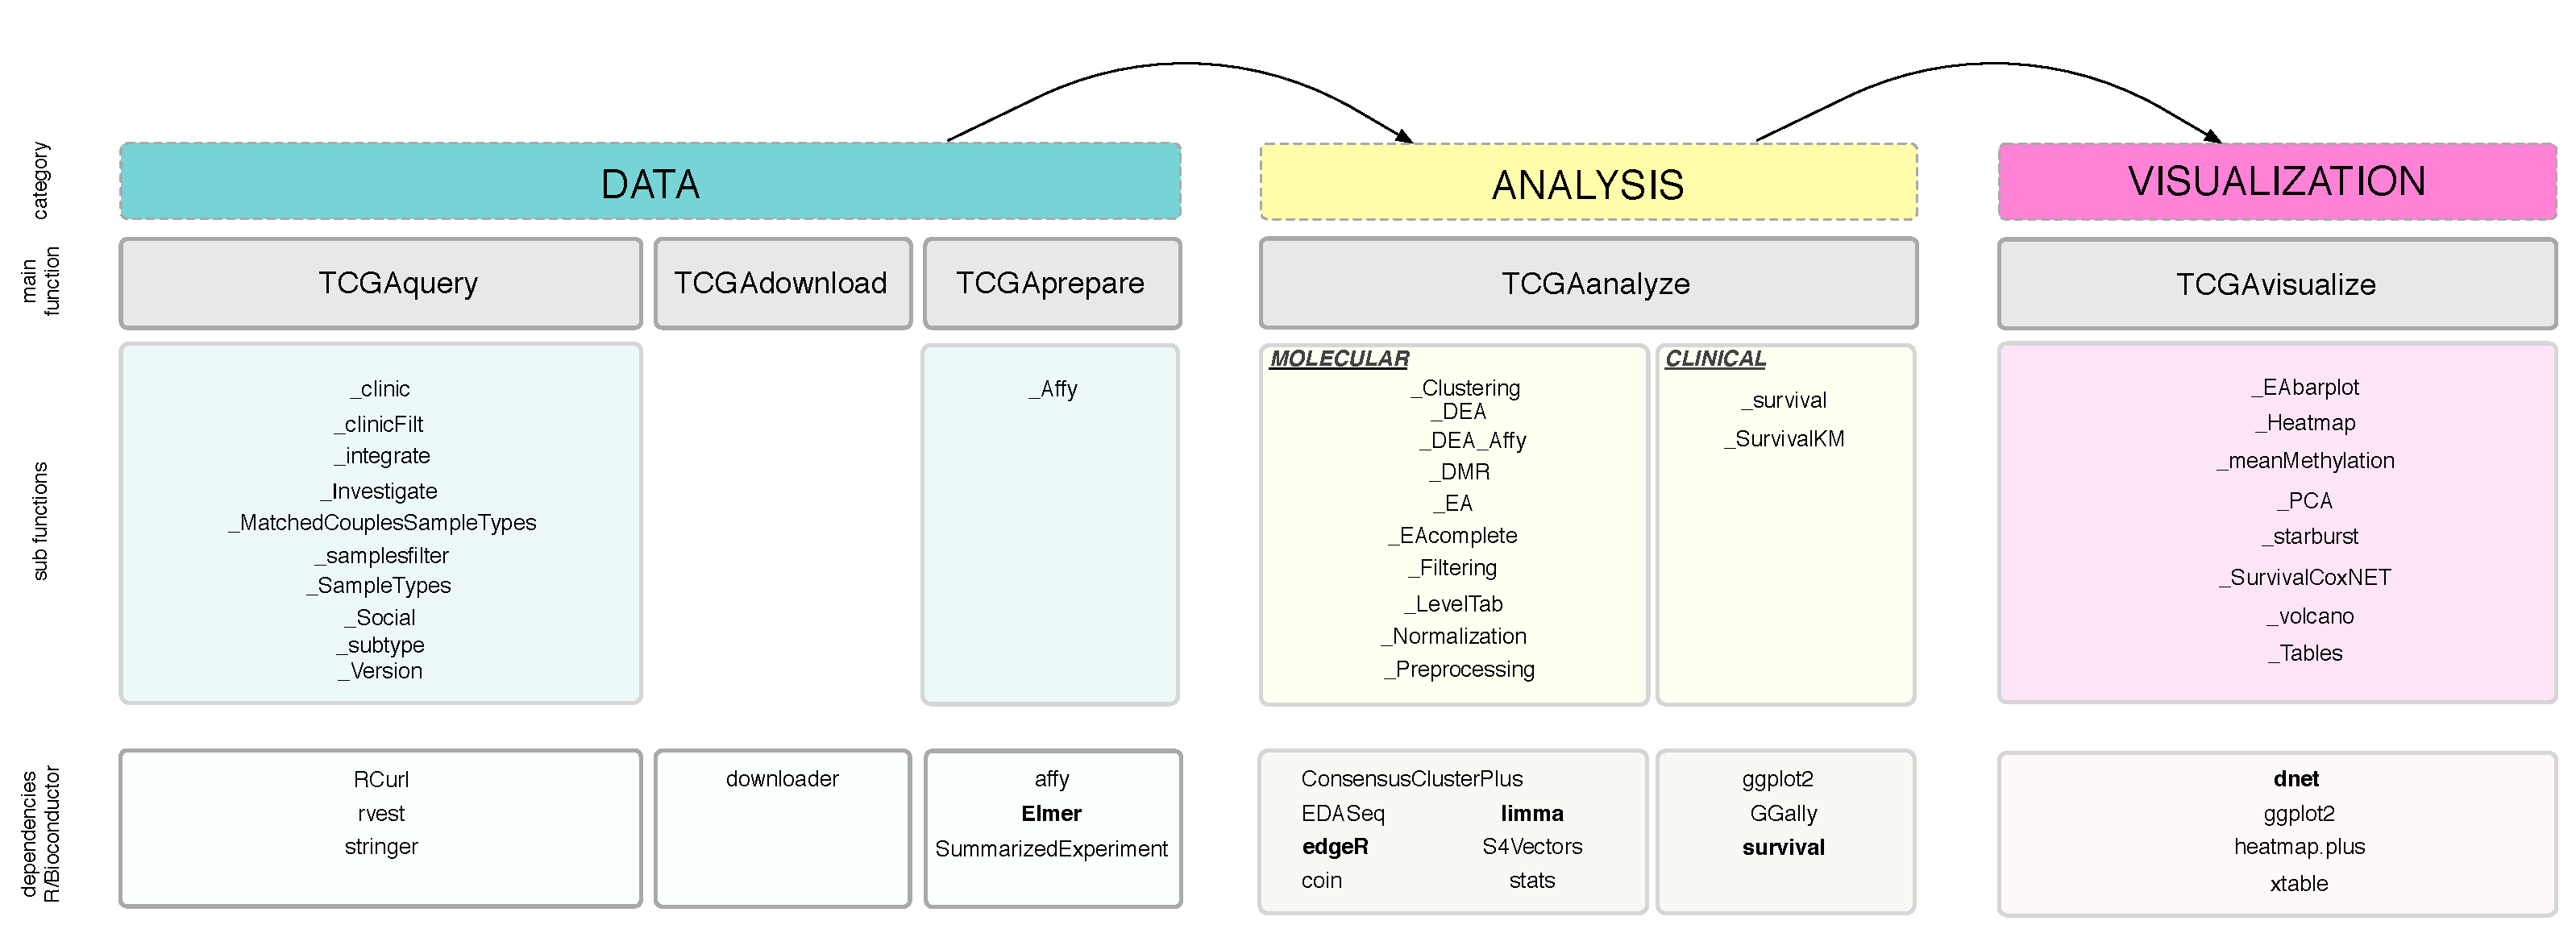
\includegraphics[width=\textwidth]{images/workflow_draft2_noboxes.pdf}
\caption{TCGAbiolinks is organized in three categories. In the first category (DATA), functions to query the TCGA database, to download the data and to prepare it are made available. The second category (ANALYSIS) contains functions that allow the user to carry out different types of analyses, these incluse clustering (TCGAanalyze\_Clustering), differential expression analysis (TCGAanalyze\_DEA) and enrichment analysis (TCGAanalyze\_EA). Finally, the obtained results can be visualized using the functions in the third category (VISUALIZATION): these include principal component analysis (TCGAvisualize\_PCA), starburst plots (TCGAvisualize\_starburst) and survival curved (TCGAvisualize\_SurvivalCoxNET). The different dependencies to other R/Bioconductor packages are named in the last row of the figure.}
\label{fig:workflow}
\end{figure*}
%With our new R package, called \textit{TCGAbiolinks}, we proposed some solutions for bioinformaticians to save their (researcher and computational) time, trying  to address the needs of both groups as follows.
%See TCGAbiolinks Bioconductor user’s guide for a more detailed description.

TCGAbiolinks simplifies access, preparation and downstream analysis of cancer data by providing high-level functions
which warp different packages as reported in the table below:  
%In the following table we reported the functions for each layer and related package used / wrapping.

% \begin{table}[ht]
% \centering
% \begin{tiny}
% \begin{tabular}{lll}
% \hline
% Layer & Function & Package used (wrapping)  \\ 
% \hline
% \cellcolor{cyan}query & TCGAquery\_clinic & RCurl \\ 
% \cellcolor{cyan}query & TCGAquery\_clinicFilt & \\ 
% \cellcolor{cyan}query & TCGAquery\_integrate & \\ 
% \cellcolor{cyan}query & TCGAquery\_MatchedCoupledSampleTypes & \\ 
% \cellcolor{cyan}query & TCGAquery\_samplesfilter & \\ 
% \cellcolor{cyan}query & TCGAquery\_SampleTypes RCurl & \\ 
% \cellcolor{cyan}query & TCGAquery\_Version & rvest, stringr \\ 
% \cellcolor{cyan}query & TCGAquery & downloader\\ 
% & & \\
% \cellcolor{yellow}download & TCGAdownload & \\ 
% & & \\
% \cellcolor{brightgreen}prepare & TCGAprepare & SummarizedExperiment, Elmer \\ 
% & & \\
% \cellcolor{coolgrey}analyze & TCGAanalyze\_DEA & edgeR\\ 
% \cellcolor{coolgrey}analyze & TCGAanalyze\_DMR & ggplot2, SummarizedExperiment,S4Vectors \\ 
% \cellcolor{coolgrey}analyze & TCGAanalyze\_EA & stats &\\ 
% \cellcolor{coolgrey}analyze & TCGAanalyze\_EAcomplete &\\ 
% \cellcolor{coolgrey}analyze & TCGAanalyze\_Filtering &\\ 
% \cellcolor{coolgrey}analyze & TCGAanalyze\_LevelTab & \\ 
% \cellcolor{coolgrey}analyze & TCGAanalyze\_Normalization & EDASeq\\ 
% \cellcolor{coolgrey}analyze & TCGAanalyze\_Preprocessing & grDevices \\ 
% \cellcolor{coolgrey}analyze & TCGAanalyze\_survival & GGally,survival,scales  \\ 
% \cellcolor{coolgrey}analyze & TCGAanalyze\_SurvivalKM & survival \\ 
% & & \\
% \cellcolor{darkorange}visualize & TCGAvisualize\_EAbarplot & \\ 
% \cellcolor{darkorange}visualize & TCGAvisualize\_meanMethylation & ggplot2, SummarizedExperiment\\ 
% \cellcolor{darkorange}visualize & TCGAvisualize\_PCA & \\ 
% \cellcolor{darkorange}visualize & TCGAvisualize\_starburst & \\ 
% \cellcolor{darkorange}visualize & TCGAvisualize\_SurvivalCoxNET & dnet\\ 
% & & \\
% \cellcolor{red}investigate & TCGAinvestigate & RCurl\\ 
% & & \\
% \cellcolor{bleudefrance}social & TCGAsocial & \\

% \hline
% \end{tabular}
% \end{tiny}
% \caption{TCGAbiolinks proposed functions and related wrapping packages} 
% \label{table:01}
% \end{table}

\subsection{TCGAQuery}

This functions is the core of the package that allows user to query data from the TCGA portal. 
%This function allows user to query TCGA about different datatypes and different platforms.
The  TCGA portal provides data  for 24 cancer and   7 different datatypes  (clinical,  mRNA,SNP, Protein, miRNA,
Methylation, Exome) using several platform.
Data in TCGA are organized in 4 levels: 1) raw, 2) processed, 3) interpreted, and 4) region of interest. The user can access to all level, if TCGA site do not require user certification for data access.
TCGAQuery allows to programmatically interrogate the  available data in terms of:
tumor, platform, samples (barcode list), level, center and version.


%\lstinputlisting{Rcode/TCGAquery_Rscripts.R}


%\begin{lstlisting}[language=R]
%query <- TCGAquery(tumor = c("gbm","lgg"), platform=Exome)
%\end{lstlisting}

In above example we reported several example of TCGAquery functions and relative subfunctions that call TCGAquery.

will return the list of available samples with exome sequencing for the Lower Grade Glioma and Glioblastoma tumor types.
More advanced queries can be created by specifying other parameters such as level, center and others.
The return type of TCGAQuery is a list of lists, the package also provides higher level query functions (Table 1) 
which manipulate such lists. For example the TCGAquery\_clinic allows to create a table from the clinical information 

%BRCAclinic <- TCGAquery_clinic(cancer = "BRCA",clinical_data_type = "clinical_patient")

% dim(BRCAclinic)

%what gives in putput
and TCGAquery\_SampleTypes allows to filter for sample types, for example to download the list of EXOME samples of recurrent tumors for Glioblastoma

% Add an example to download Recurrent tumor of Glioblastoma GBM

%SS <- TCGAquery_SampleTypes(bar,c("TR","TRBM"))

% See table \ref{TCGAQueryoutput}

%TCGA's data are organized according datatype and platform about 24 cancers.
%In particular there are several samples with identification of TCGAbarcode
%that it is composed by 16 chrs.


%Clinical data are important because it can be used for different analysis
%like survival analysis and also to retrieve information about samples like drugs, follow up, stages, and also molecular subtypes.


\textit{TCGAquery\_clinic} 
This functions is used to query and retrieve informations about samples available in TCGA data portal see for example Fig~\ref{NAR-fig5}.

% \begin{figure}[!h]
% \begin{center}
%   \includegraphics[width=.9\linewidth]{images/clinicData2.png}
%   \end{center}
%   \caption{Example of clinical patient's data for BRCA cancer}
%   \label{NAR-fig5} % \label{fig:sfig2}
% \end{figure}

\textit{TCGAquery\_clinicFilt} 
With this function the user will filter the data, returning the list of barcodes that matches all the filter.
The information that can be retrieved are about 
\begin{tiny}
\begin{itemize}[nolistsep]
\item positive or negative her2 neu immunohistochemistry receptor status. 
\item gender, MALE or FEMALE
\item Positive or Negative Progesterone receptor status.
\item stage, Pathologic Stage: stageIX, stageI, stageIA, stageIB, stageIIX,stageIIA, stageIIB, stageIIIX,stageIIIA, stageIIIB, stageIIIC, stageIV.
\item Positive or Negative Estrogen receptor status.
\end{itemize}
\end{tiny}


\textit{TCGAquery\_samplesfilter} 
As shown in TCGAquery Rcode examples, this function help the researcher for filtering sample output from TCGAquery.

%\begin{enumerate}[topsep=0pt,itemsep=-1ex,partopsep=1ex,parsep=1ex]
\textit{TCGAquery\_integrate} 

Some times researches would like to use samples from different platforms 
from the same patient. In order to help the user to have an overview of the number of samples in commun we created this function that will receive the data frame returned from TCGAquery and produce a matrix n platforms x n platforms with the values of samples in commum.
This function creates a table with common samples analyzed with different platforms (e.g. matched miRNA-mRNA), that can be used in two by two comparison to retrieve a list of common samples (TCGA barcode) that can be downloaded saving time. 

The result of the 3 platforms for BRCA is shown below:

\begin{table}[!h]
\centering
\begin{tiny}
\begin{tabular}{llll}

  \hline
& AgilentG4502A\_07\_3 & HumanMethylation450 & IlluminaHiSeq\_RNASeqV2 \\ 
\hline
AgilentG4502A\_07\_3 & 604 & 224 & 530 \\ 
HumanMethylation450 & 224 & 930 & 790 \\ 
IlluminaHiSeq\_RNASeqV2 & 530 & 790 & 1218 \\ 
   \hline
\end{tabular}
\end{tiny}
\caption{Table common samples among platforms from TCGAquery} 
\label{table:02}
\end{table}


% We can integrate the function TCGAquery_MatchedCoupledSampleTypes in TCGAquery_SampleTypes adding some parameters and using only 1 functions for samples Types.

\textit{TCGAquery\_SampleTypes} 
This functions allows user to retreive informations about samples for example: TP, TN, etc. % add more informations
It is possible to retrieve multiple tissue types from the same patients or different one.
This function allows user to obtain a list of barcodes with a specific clinical data. For instance the user can indicate tissue type to download (primary, recurrent,metastatic,..), in case of multi tissue types can define matched sample from the same patients
\begin{table}[!h]
\centering
\begin{tiny}
\begin{tabular}{ll}
  \hline
typesample &  tissue type definition \\ 
\hline
TP &   PRIMARY SOLID TUMOR \\
TR &   RECURRENT SOLID TUMOR \\
TB &   Primary Blood Derived Cancer-Peripheral Blood \\
TRBM & Recurrent Blood Derived Cancer-Bone Marrow \\
TAP &  Additional-New Primary \\
TM &   Metastatic \\
TAM &  Additional Metastatic \\
THOC & Human Tumor Original Cells \\
TBM &  Primary Blood Derived Cancer-Bone Marrow \\
NB &   Blood Derived Normal \\
NT &   Solid Tissue Normal \\
NBC &  Buccal Cell Normal \\
NEBV & EBV Immortalized Normal \\
NBM &  Bone Marrow Normal \\
  \hline
\end{tabular}
\end{tiny}
\caption{Table with tissue type definition from TCGAquery} 
\label{table:03}
\end{table}


\subsection{TCGADownload}
TCGA's cancer data as organized in table (add) has stored on ftp site and typically and in table are reported average of size of data for each cancer and platform type.
{\color{red} Give the idea of dimension of file in GByte for each platform}
It is important the selection of only file that user need for next steps such as preparion and analysis.

The TCGAdownload function will download the data using as reference the the lines of the TCGAquery search result. 
There is an option to download the entire tar.gz folder or download specific files using the \emph{type} parameter or the \emph{samples} parameter
The output files will be saved into the path parameters. If this path does not exists the package will try to create the directories. By default, if a sample was already downloaded the function will not download again, unless the force parameter is set to \emph{TRUE}
TCGAdownload allows also to download only a list of samples as output of TCGAQuery, eg. selecting level (1,2,3) common samples between two or three platforms. 

\begin{tiny}
\begin{itemize}[nolistsep]
\item data The TCGAquery output
\item path Directory to save the downloaded data
\item type Filter the files that will be downloaded by Example:"rsem.genes.results"
\item samples List of samples to download data
\item force Download files even if it was already downladed?
\end{itemize}
\end{tiny}

\subsection{TCGAPrepare}
The TCGAPrepare function will read the data from level 3 the experiments and prepare it for downstream analysis into a SummarizedExperiment object. The samples are always refered by their barcode. If you want to save the data into an rda file, please use the \emph{save}
parameter that will save an rda object with the  \emph{filename} parameter.
If no filename was set, the filename will be the concatenation of platform and Sys.time.
You can easily read the downloaded data using the `TCGAprepare` function.
This function will prepare the data into a SummarizedExperiment

\url{http://www.nature.com/nmeth/journal/v12/n2/abs/nmeth.3252.html}
object for downstream analysis. 
For the moment this function is working only with data level 3.

The arguments are:
\begin{tiny}
\begin{itemize}[nolistsep]
\item query**	Data frame as the one returned from TCGAquery
\item dir**	Directory with the files
\item type**	File to prepare.
\item samples**	List of samples to prepare.
\item save**	Save a rda object with the prepared object? Default: FALSE
\item filename** Name of the rda object that will be saved if `save` is `TRUE`
\item toPackage** Name of the package to prepare the data specific to that package. 
\item summarizedExperiment** Should the output be a SummarizedExperiment object? Default: `TRUE`
\item reannotate** Reannotate genes? Source http://grch37.ensembl.org/. 
Default: `FALSE`. (For the moment only working for methylation data)
\end{itemize}
\end{tiny}

In order to add useful information to researchers we added in the colData of the 
summarize can be found in the section of most recent TCGA's publication.
\url{https://tcga-data.nci.nih.gov/docs/publications/}

We intend to add more tumor types in the future.
Also in the  metadata of the objet we added the parameters used in TCGAprepare,
the query matrix used for preparing, and file information (name,creation time and modification time) in order to help the user know which samples, versions, and parameters they used.

As an example, for the platform IlluminaHiSeq\_RNASeqV2 we prepared  samples for the rsem.genes.normalized\_results type. In order to create the object mapped the gene\_id 
to the hg19. The genes\_id not found are then removed from the final matrix.
The default output is a SummarizedExperiment is shown below. 

In order to create the SummarizedExperiment object we mapped the rows of the 
experiments into GRanges. In order to map miRNA we used the miRNA from the anotation database TxDb.Hsapiens.UCSC.hg19.knownGene, this will exclude the miRNA from viruses and bacteria. 
In order to map genes, genes alias, we used the biomart hg19 database 
(hsapiens\_gene\_ensembl from grch37.ensembl.org).

In case you prefere to have the raw data. You can get a data frame without any
modification setting the `summarizedExperiment` to false. Table of `types` available for the `TCGAprepare`.

Preparing the data with parameter \textit{toPackage} 
This section will show how to integrate `TCGAbiolinks` with other packages.
Our intention is to provide as many integrations as possible.

The example below shows how to use `TCGAbiolinks` with `ELMER` package 
(expression/methylation analysis). The TCGAprepare for the DNA methylation data 
will Removing probes with NA values in more than 0.80\% samples and remove the 
anotation data, for the expression data it will take the log2(expression + 1)
of the expression matrix in order to linearize the relation between 
DNA methylation and expression also it will prepare the rownames as the 
specified by the package.

%Prepare data matrices (genes/ loci in rows, samples in columns) for downstream analysis, ready to use also with other R packages such as: limma, edgeR, stats, survival, etc.. See for details Supplementary Table~\ref{table::DownstreamAnalysis}.

\begin{table}[b]
\caption{Platforms supported by TCGABiolinks.}
\label{table:01}%
}{%
\begin{tiny}
\begin{tabular*}{\columnwidth}{@{}lll@{}}
\toprule
dataType  &  Platform & File type
\\
mRNA & agilentg4502a 07 1 & \\
mRNA & agilentg4502a 07 2 & \\
mRNA & agilentg4502a 07 3 & \\
mRNA & hg-u133 plus 2 & \\
mRNA & ht hg-u133a & \\
mRNA & huex-1 0-st-v2 & \\
mRNA & illuminaga mrna dge & \\  
mRNA & illuminaga rnaseq & exon.quantification, spljxn.quantification,  gene.quantification\\
mRNA & illuminaga rnaseqv2 & junction\_quantification, rsem.genes.results, rsem.isoforms.results, rsem.genes.normalized\_results, rsem.isoforms.normalized\_results, bt.exon\_quantification \\
mRNA & illuminahiseq rnaseq & \\
mRNA & illuminahiseq rnaseqv2 & \\
mRNA & illuminahiseq totalrnaseqv2 & \\
toChange & genome\_wide\_snp\_6 & hg18.seg,hg19.seg, nocnv\_hg18.seg, nocnv\_hg19.seg \\
mRNA & agilentg4502a 07 1 & \\
mRNA & agilentg4502a 07 2 & \\
mRNA & agilentg4502a 07 3 & \\
\end{tabular*}%
\end{tiny}
\end{table}

\subsection{TCGAnalyze}



The analysis part of TCGAbiolinks package incorporate several statistical methods 
for fast analysis of \textit{omic} data from TCGA's portal.
This allows for example reducing number of features to a signature of genes that can discriminate between dead or alive for survival or between normal and tumor samples, etc.
For each analytical functions, downstream analysis from modified published vignette and time evaluation analysis methods are provided and are available in Supplementary table.

Analyze data matrices (genes/ loci in rows, samples in columns) for downstream analysis, ready to use also with other R packages, like differential expression analysis, classification, ROC, AUC, inference of gene regulatory network, feature selection, survival analysis, enrichment analysis, and master regulator analysis.

\textit{TCGAanalyze\_DEA}

The most common goal among investigators using either microarrays or RNA-seq is detecting differential expression, for example: discovering transcripts showing different average expression levels across two populations.
Frequently the important investigations with microarrays and rnaseq's data are to identify the genes whose expression levels change between two sample groups. To understand the effect of a drug we may ask which genes are up-regulated (increased in expression) or down-regulated (decreased in expression) between treatment and
control groups.

DEA (Differential expression analysis) to identify differentially expressed genes (DEGs) is performed using the `TCGAanalyze\_DEA` function. 

To determine whether a gene is expressed in a differential manner, we apply a test of hypothesis and the fold-change between the two starting conditions, in tumor and normal. In particular we use the edgeR package from Bioconductor that uses the quantile-adjusted conditional maximum likelihood (qCML) method for experiments with single factor to determine genes differentially expressed \cite{Robinson2010}. Compared against several other estimators, qCML is the most reliable in terms of bias on a wide range of conditions and specifically performs best in the situation of many small samples with a common dispersion. The p-values generated from the analysis sorted in ascending order, are corrected using the Benjamini-Hochberg procedure for multiple testing correction.

After DEA it is possible to filter the output of dataDEGs by abs(LogFC) >=1, and uses the `TCGAanalyze\_LevelTab` function to create a table with DEGs (differentially expressed genes), log Fold Change (FC), false discovery rate (FDR), the gene expression level for samples in Cond1type, and Cond2type, and Delta value (the difference of gene expression between the two conditions multiplied logFC).

\subsection{TCGAVisualize}
Visaulize is an important part of the package.
Data visualization tools for gene expression and methylation analysis such as Heatmap, cluster and several plots, pathway enrichment analysis.

\subsection{Case study 3b: Downstream Analysis Integration of Gene Expression and Methylation data}


In this section we consider a case study with methylation and expression data from COAD samples. 


\begin{figure*}
\centering
%\includegraphics[width=.9\linewidth]{figures/case3_improved.pdf}
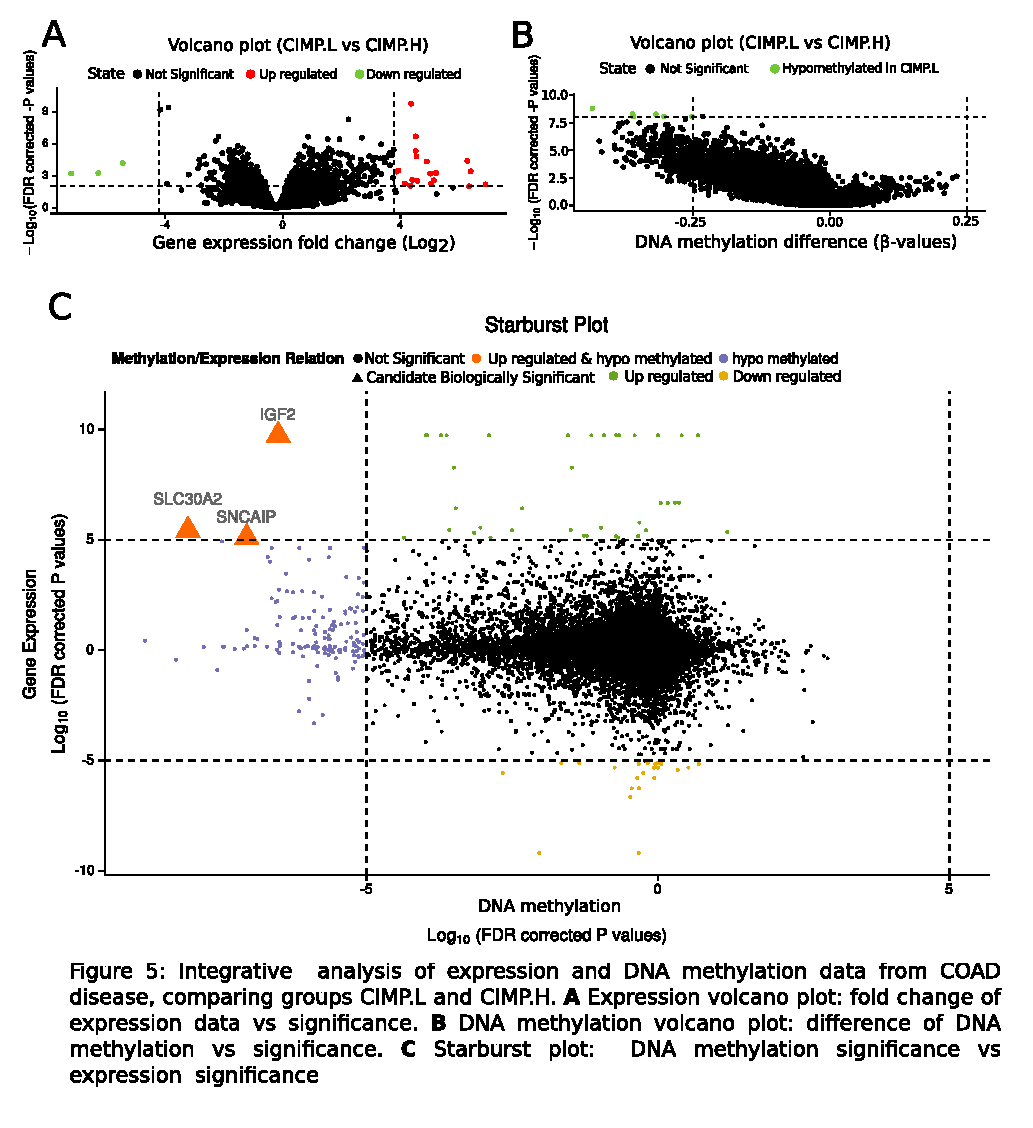
\includegraphics[width=.9\linewidth]{images/case3_improved2.pdf}

\caption{Integrative analysis of expression and DNA methylation from COAD disease}
\label{fig:workflow}
\end{figure*}

\newpage